\documentclass[
    11pt,
    a4paper,
    sfdefaults=false,
    toc=chapterentrywithdots,
    twoside,openright,
    titlepage,
    parskip=half,
    headings=normal,  % reduces heading size
    listof=totoc,
    bibliography=totoc,
    index=totoc,
    captions=tableheading,  % caption below table
    chapterprefix,
    listof=flat,
    final,
    openany
]{scrbook}


% details about your thesis
\newcommand{\titel}{Automatische Generierung von Themenspezifischen Podcasts aus einer großen Audiodatenbank}
\newcommand{\artderarbeit}{Bachelorarbeit}  % {Bachelorarbeit,Masterarbeit}
\newcommand{\autor}{Vincent Neumann}
\newcommand{\studiengang}{Medieninformatik}  % {Informatik,Wirtschaftsinformatik,Medieninformatik}
\newcommand{\matrikelnr}{358\,5287}
\newcommand{\erstgutachter}{Prof.\,Dr.~Florian Gallwitz}
\newcommand{\zweitgutachter}{Prof.\,Dr.~Anna Kruspe}
\newcommand{\betreuer}{~Florian Thoma}
\newcommand{\unternehmen}{Public Value Technologies GmbH}
\newcommand{\logo}{figures/TH-Nuernberg-RGB.png}
\newcommand{\keywords}{hot, fuzz}
 

% custom head and foot
\usepackage[automark]{scrlayer-scrpage}
\pagestyle{scrheadings}
\ihead{\headmark}
\chead{}
\ohead{\pagemark}
\renewcommand*\chaptermarkformat{\chapappifchapterprefix{\ }% 
  \thechapter.\enskip}

\RedeclareSectionCommand[tocindent=0pt]{section}
\RedeclareSectionCommand[tocindent=0pt]{subsection}
%\RedeclareSectionCommand[tocnumwidth=70pt]{chapter}

\usepackage{scrhack}

% other packages
\usepackage[utf8]{inputenc}
\usepackage[T1]{fontenc}
\usepackage{lmodern,relsize,textcomp,csquotes}
\usepackage{amsmath,amsfonts}
\usepackage[ngerman,english]{babel}  % flip for German thesis
\usepackage[final]{graphicx}
\usepackage{setspace,geometry,xcolor}
\usepackage{makeidx}
\usepackage{paralist,ifthen,todonotes}
\usepackage{url}
\usepackage[toc]{glossaries}
\usepackage{pdfpages}
\usepackage{amsmath}

% table setup
\usepackage{longtable}
\usepackage{array}
\usepackage{ragged2e}
\usepackage{lscape}

% pdf hyperref
\usepackage[
    bookmarks=true,
    bookmarksopen=true,
    bookmarksnumbered=true,
    bookmarksopenlevel=1,
    pdftitle={\titel},
    pdfauthor={\autor},
    pdfcreator={\autor},
    pdfsubject={\titel},
    pdfkeywords={\keywords},
    pdfpagelabels=true,
    colorlinks=true,
    linkcolor=red,
    urlcolor=magenta,
    anchorcolor=black,
    citecolor=cyan,
    filecolor=magenta,
    menucolor=red,
    plainpages=false,
    hypertexnames=true,
    linktocpage=true,
]{hyperref}

% biblatex
% \usepackage[backend=biber, style=authoryear]{biblatex}
\usepackage{biblatex}
% \addbibresource{literatur.bib}

% configure your listings style
\usepackage{listings}
\lstset{
	tabsize=3,
	extendedchars=true,
	frame=single,
	showstringspaces=true,
	numbers=left,
	numberstyle=\small,
	breakautoindent=true
}

% page setup
% \setlength{\topskip}{\ht\strutbox}
\geometry{paper=a4paper,left=2.5cm,top=3.0cm,bindingoffset=.8cm}
\onehalfspacing
\frenchspacing
\clubpenalty = 10000
\widowpenalty = 10000 
\displaywidowpenalty = 10000

% some commands
\newcommand{\ua}{\mbox{u.\,a.\ }}
\newcommand{\zB}{\mbox{z.\,B.\ }}
\newcommand{\dahe}{\mbox{d.\,h.,\ }}
\newcommand{\bzw}{\mbox{bzw.\ }}
\newcommand{\bzgl}{\mbox{bzgl.\ }}
\newcommand{\eg}{\mbox{e.\,g.\ }}
\newcommand{\ie}{\mbox{i.\,e.\ }}
\newcommand{\wrt}{\mbox{w.\,r.\,t.\ }}
\newcommand{\etal}{\mbox{\emph{et.\,al.\ }}}


% TODO remove if not needed...
\usepackage{blindtext}

% load glossary entries
\makenoidxglossaries
\loadglsentries{glossary}

\addbibresource{literatur.bib}

\begin{document}

\setcounter{secnumdepth}{3}  % numerate subsections
\setcounter{tocdepth}{2}  % ...but don't include them in toc

\frontmatter
\thispagestyle{empty}
\pdfbookmark[1]{Cover}{cov}
\begin{titlepage}

\begin{center}

\includegraphics[width=\linewidth]{figures/ohm-logo.png}\\[1cm]
\LARGE{Fakultät Informatik}\\[2cm]

\huge
\textbf{\titel}\\[1cm]
%
\Large
\artderarbeit~im Studiengang \studiengang\\[1cm]
%
\large
vorgelegt von

\Large
\autor\\[0.5cm]
\small
Matrikelnummer \matrikelnr\\[2cm]

\vspace*{\fill}

\large
\begin{tabular}{p{3cm}p{8cm}}\\
Erstgutachter:  & \quad \erstgutachter\\[1.2ex]
Zweitgutachter: & \quad \zweitgutachter\\[1.2ex]
%discomment "Betreuer" and "Unternehmen" for a thesis in a company
Betreuer: & \quad \betreuer\\
Unternehmen: & \quad \unternehmen
\end{tabular}
\end{center}

\begin{center}
\copyright\,\the\year
\end{center}

\vspace{-0.5cm}
\singlespacing
\small
\noindent Dieses Werk einschließlich seiner Teile ist \textbf{urheberrechtlich geschützt}.
Jede Verwertung außerhalb der engen Grenzen des Urheberrechtgesetzes ist ohne Zustimmung des Autors unzulässig und strafbar.
Das gilt insbesondere für Vervielfältigungen, Übersetzungen, Mikroverfilmungen sowie die Einspeicherung und Verarbeitung in elektronischen Systemen.

\end{titlepage}
\cleardoublepage

% download the following form and complete it (hit save in your editor)
% https://intern.ohmportal.de/fileadmin/Gelenkte_Doks/Abt/SZS/SB/SB_0050_FO_Pruefungsrechtliche_Erklaerung_und_Erklaerung_zur_Veroeffentlichung_der_Abschlussarbeit_public.pdf
%\includepdf{SB_0050_FO_Pruefungsrechtliche_Erklaerung_und_Erklaerung_zur_Veroeffentlichung_der_Abschlussarbeit_public.pdf}\cleardoublepage

\thispagestyle{empty}
\section*{Kurzdarstellung}
\label{sec:kurzdarstellung}

In dieser Arbeit wird ein Ansatz für die automatische Erstellung einer Podcastepisode aus vorhandenem Audiomaterial vorgestellt. 
Dafür wird ein umfangreiches System aus mehreren Microservices erstellt, das den kompletten Verlauf von der Beschaffung der Audiodaten bis zur Bereitstellung einer Podcastepisode in einem User-Interface abdeckt.






\cleardoublepage

\tableofcontents

\mainmatter
\pagenumbering{arabic}
\chapter{Einleitung}\label{ch:intro}

\section{Motivation}

Podcasts sind für viele Menschen ein wichtiges Medium, um sich die Zeit zu vertreiben und sich über verschiedene Themen zu informieren. 
In Deutschland hören ca. 29\% der Menschen regelmäßig Podcasts \cite{newman2022}.
Dabei liegt die Nutzung der ARD-Audiothek mit 12\% auf Platz drei hinter Spotify und Youtube[TODO Quelle].
Wie Studien gezeigt haben, verbessert sich das Audioerlebnis der Zuhörer*innen dabei, wenn mehrere verschiedene Sprecher*innen dabei vorkommen \cite{kang2012}. 
Einige Podcasts werden zum Beispiel nur von einer einzigen Person vorgetragen.
Außerdem steigert das Vorhandensein verschiedener Meinungen auch das Interesse des Zuhörers an einem bestimmten Thema \cite{phillips2014}.
Neben diesen Vorteilen, ist es für die Zuhörer*innen einer Podcast Episode auch ein besonderer Aspekt der Selbstbestimmung, wenn sie die Länge einer Podcast Episode selbst festlegen können.
In dieser Arbeit wird es darum gehen, wie man diese Vorteile einer personalisierten Podcast Episode ausnutzen kann.


\section{Zielsetzung}


Das Ziel dieser Bachelorarbeit besteht darin zu untersuchen, wie sich aus umfangreichem Audiomaterial aus Radioprogrammen oder Podcasts on-the-fly ein eigener Podcast zusammenstellen lässt, der relevante Ausschnitte aus einer Vielzahl von Audiomaterial enthält.

Ein möglicher Anwendungsfall wäre ein/e Benutzer*in, die/der sich über das Thema "Überfischung der Meere" informieren möchte und dafür genau 20 Minuten während einer Autofahrt einplant. 
Das System erstellt nun einen Zusammenschnitt aus verschiedenen Podcast Episoden zu diesem Thema, der 20 Minuten lang ist und stellt ihn dem/der Benutzer*in zur Verfügung. 
Der Vorteil für den/die Nutzer*in liegt darin, dass er/sie selbst das Thema auswählen und die exakte Länge festlegen kann, um beispielsweise während einer 20-minütigen Autofahrt einen Podcast anzuhören. 
Außerdem werden das Thema von verschiednen Personen aus unterschiedlichen Blcikpunkten erklärt. 

Für die Interaktion mit dem Benutzer soll außerdem eine Grafische Benutzeroberfläche bereitgestellt werden, die dem Nutzer die Auswahl eines Themas und die Länge der Podcast  Episode ermöglicht.

\section{Überblick}

Im zweiten Kapitel werden theoretische Grundlagen zum Verständnis der später aufgeführten Technologien erklärt.

Im dritten Kapitel wird es um die Beschaffung der Datengrundlage gehen. Als Datenquelle werden Podcast Episoden aus der Audiothek der ARD benutzt. 
Dann werden verschiedene Methoden zur Transkription dieser Audiodaten beschrieben und begründet, welche Wahl der Transkription für diese Arbeit verwendet wird.

Im vierten Kapitel wird die Architektur des Systems dargestellt. 
Dabei wird besonders auf die semantische analyse der Transkriptionen eingegangen und verschiedene Aspekte des Natural Language Processing und der Large Language Models vorgestellt.

Im fünften Kapitel werden verschiedene Methoden zur semantischen Analyse evaluiert.
Dabei werden auch die verwendeten Modelle die Wahl der Anzahl und Länge der Abschnitte und die finale Zusammensetzung dieser Abschnitte erklärungt und begründet.

Im sechsten Kapitel wird ein Ausblick auf zukünftige Verbesserungen gegeben.

Im siebten Kapitel wird eine Zusammenfassung der erzielten Ergebnisse gegeben.

\chapter{Ausgangslage und theoretische Grundlagen}\label{ch:data}

\section{Ausgangslage}
 
Die Podcastbranche wächst seit vielen Jahren stetig und immer mehr Menschen hören regelmäßig Podcasts 
In Deutschland ist die ARD Audiothek ein großer Podcastanbieter mit mitlerweile über 41 Millionen Audioabrufen und über 80.000 verschiedenen Audioinhalten zum Abrufen. Auch die Zahlen der Audiotheksbenutzer, sowie der App-downloads steigen weiterhin. \cite{gotting2023}

Gleichzeitig wächst auch der Markt an AI-basierten Podcasts. So erreichen heute schon AI-basierte Podcasts rund 45 Millionen US-Amerikaner 

\section{KI in Podcasts}

Künstliche Intelligenz verändert die Branche des Podcastings in vielerlei Hinsicht. 

Transkriptionsmodelle wie Whisper sind in der Lage live Transkriptionen der Podcasts zu erstellen die eine Qualität bestitzen, die mit professionellen menschlichen Transkriptoren mithalten kann \cite{radford}.
Diese können außerdem verschiedene Stimmen unterscheiden und die Emotionen der Sprecher erkennen, was es in der Nachbereitung eines Podcasts erheblich erleichtert bestimmte Stellen zu finden \cite{wagner2023}
Ein großes Entwicklungsfeld in der Podcastbranche ist die komplett automatische Generierung von Podcasts. Die Technologie der automatischen Stimmengenerierung ist soweit fortgeschritten, dass sich künstlich generierte Stimmen fast so gut anhören wie echte Stimmen \cite{shi2023}.


\section{Embeddings}

Das Ziel dieser Arbeit besteht darin, eine Schnittstelle für einen Hörer zu erstellen, die ihm ermöglicht, einen Zusammenschnitt aus vielen verschiedenen Podcast Episoden ist, und genau zu einem Thema passt. 
Die wichtigste Aufgabe besteht also darin, die wesentlichen Abschnitte aus den Episoden herauszufinden. 
Bis jetzt haben wir zu jedem Audiofile eine transcript.json, bei der das Transkript in regelmäßigen Zeitabschnitten mit Zeitstempeln markiert ist. 
Die Aufgabe, auf eine Userfrage hin die wesentlichsten Segmente herauszufinden lässt sich auf mehrere Arten lösen. 
Dazu werden wir verschiedene Verfahren aus der Wissenschaft im Bereich Natural Language Processing (NLP) verwenden.

\section{Motivation für Embeddings}

Die menschliche Sprache ist ein hochkomplexes Konstrukt mit einer Grammatik, die sehr viel flexibler, kreativer, vieldeutiger, und komplexer ist als maschinensprache. 
Es gibt viele kleine Bedeutungsnuancen, sie ist stark von dem allgemeinen Wissen der Welt geprägt und sie ändert sich im laufe der Zeit. 
Das alles macht es für Computer sehr schwierig die Menschliche Sprache zu Verstehen. 
Neuere Forschung im Bereich des Natural Language Processing bietet einige Ansätze um dieses Problem zu lösen. 
Es gibt dazu viele verschiedene Methoden, die alle darauf abzielen, Worte oder Texte in Vektoren umzuwandeln, die den Inhalt dieser Worte oder dieser Texte repräsentiert.
Diese Vektoren nennt man Embeddings.
Das Ziel dieser Embeddings besteht für unseren Zweck darin, eine Suchfunktion zu beschreiben, die auf eine Anfrage (Query) hin, passende Dokumente aus einem großen Korpus an Dokumenten liefern kann.

Die Geschichte der Embeddings startet mit stochastischen Verfahren, wie TF-IDF und BM25. 
Term Frequency - inverse Dokument Frequency (TF-IDF) ist ein Algorithmus um Dokumente nach Keyworten zu durchsuchen.
Das Verfahren verwendet Worthäufigkeiten (Term-Frequency), um Dokumenten, in denen ein Wort häufiger vorkommt zu bevorzugen.
Außerdem verwendet es die generelle Seltenheit von Wörter (Inverse Document Frequency) um Wörtern, die seltener vorkommen mehr Gewicht bei der Suche einräumen.

Daraus bildet der TF-IDF Algorithmus einen dünnbesetzten Vektor, der die Anzahl und Seltenheit jedes im Dokument vorkommendes Wortes abbildet. 
Dünnbesetzt heißt in diesem Zusammenhang, dass der Vektor viele Einträge mit dem Wert 0 besitzt. 
Das folgt aus der Bedingung, dass diese Vektoren untereinander vergleichbar sein müssen und dadurch Einträge für jedes Wort besitzen, welches im gesamten Korpus an Dokumenten vorkommt.
Jedes einzelne Dokument hat dabei aber nur ein Bruchteil der Gesamtwörter und damit viele Nullwerte.

Best Matching 25 (BM25) ist eine Famile von Algorithmen die versuchen den TF-IDF Algorithmus zu verbessern indem sie versuchen, die Priorisierung Langer Dokumente und zu oft vorkommende Worte auszugleichen.

Außerdem kann man diese Algorithmen noch anpassen, sodass sie auch n-gramme als Einträge der Vektoren miteinbeziehen. 
Das heißt, dass nicht nur einzelne Wörter berücksichtigt werden, sondern auch häufig zusammen vorkommende Wörter als einzelnes Token in dem Vektor abgebildet werden. 
Das bewirkt zwar, dass die Ähnlichkeit der Dokumente in der Regel besser ermittelt werden kann, vergrößert aber die Vektoren überproportional.

Semantische Analysen begannen erst ab ca. 1990 mit der Latenten Semantischen Analyse (LSA).
Diese verwendet Eigenvektoren um aus einer Term-Frequency Matrix versteckte (latente) Eigenschaften zu ermitteln, welche die Dokumente besser repräsentieren als die TF Matrix an sich. 
Es werden von diesen Eigenvektoren nur die wichtigsten ausgewählt, sodass jedes Dokument sehr gut als eine linearkombination dieser Vektoren repräsentiert werden kann.
Dann werden nur noch die Koeffizienten dieser Vektoren gespeichert und man kann von einer Dimensionsreduktion profitieren.
Die resultierenden Koeffizienten-Vektoren sind nun nicht mehr spärlich besetzt sondern Dicht.
Die resultierenden Eigenvektoren bilden häufig latente Themen der Dokumente ab.

Wirkliche semantische Word Embeddings kamen erst mit der Veröffentlichung von Word2Vec (2013) in den breiteren Nutzen. 
Word2Vec verwendet ein neuronales Netz, um mithilfe der benachbarten Wörter Kontextinformationen über das eigentliche Wort zu erhalten. 
Dafür gibt es die beiden Ansätze continous Bag of Words und Skipgramm.
Bei dem Ansatz Continous Bag of words werden dem Neuronalen Netz die umgebenden Wörter als Input gegeben, und das Model hat die Aufgabe daraus das Wort zu ermitteln. 
Dieses Verfahren wird in einem Sliding Window für jedes Wort aus einem Text wiederholt. 
Für einen bestimmten Korpus aus verschiedenen Dokumenten kann dieses Modell dadurch die beziehungen verschiedener Worte zueinander und die Ähnlichkeit verschieddener Worte, die oft in gleichem Kontext vorkommen erlerenen. 
Das Verfahren des Skipgramms funktioniert ähnlich, allerdings wird dabei für jedes Wort versucht die umliegenden Wörter zu ermitteln. 
Dieser Ansatz dauert länger im Training, hat aber den Vorteil, dass er auch seltener vorkommende Wörter gut repräsentieren kann.

Ein Jahr später wurde GloVe (Global Vectors for Word Representations) als Forschungsprojekt von der Stanford Universität vorgestellt. 
GloVe verbindet Konzepte aus LSA und Word2Vec, indem es die auf einer globalen Matrix Faktorisierung beruht aber die Distanz von Wörtern zueinander mitberücksichtigt.
Dadurch schaffte GloVe eine weitere Verbesserung der Embeddings und wird heutzutage noch unter anderem in NLP Bibliotheken wie SpaCy verwendet.[englische Wikipedia referiert auf Buch aus 2018]

Im Jahre 2018 wurde der Ansatz ELMo (Embeddings from Language Model) für Word Embeddings vorgestellt.
Dieser benutzt Bidirectionale Long Short Term Memory Modelle (LSTM) um daraus Embeddings zu generieren.
LSTM Modelle basieren auf Recurenten Neuronalen Netzen (RNN) und gehören zu den Sequenz to Sequenz Modellen. 
Sie bestehen dabei aus einem Encoder und einem Decoder.
Der Encoder codiert eine Inputsequenz, zum Beispiel ein Dokument, zu einem Embeddingvektor. 
Der Decoder dekodiert diesen Embeddingvektor wieder zu einer Sequenz, z.B. einer Zusammenfassung des Dokuments. [Quelle]
Für ELMo ist dabei nur der Encoder Teil wichtig.
Dabei werden zwei Layer von Forward und Backward LSTMs eingesetzt, die für jedes Wort den Kontext vor und nach dem Wort berücksichtigen, um sematische Embeddings zu erstellen. [Quellen]

Ein Jahr später wurden die Erstellung von Word und Sentence Embeddings durch BERT revolutioniert.
BERT (Bidirectional Encoder Representations from Transformers) \cite{devlin2019} ist ein auf NLP Aufgaben spezialisierter Transformer.
Das Model wurde von Google 2019 entwickelt und war seinerzeit das Beste Model, indem es in elf verschiedenen Aufgaben im Bereich des NLP State-of-the-art Ergebnisse lieferte.
Es ist auf zwei Datensätzen, dem BooksCorpus mit 800 Millionen Wörtern und der englischen Wikipedia mit 2,5 Milliarden Wörtern trainiert worden. \cite{devlin2019}
Dadurch hat BERT von einer große Auswahl an verschiedenen Themen gelernt und kann für diese sinnvolle Semantische Embedding Vektoren erstellen.













Unter diesen Aufgaben befinden sich Next Sentence Prediction (NSP) und Masked Language Modeling, auf die es auch trainiert wurde.



Außerdem kann man das Modell mit wenig aufwand auf andere Aufgaben finetunen und damit sehr gute Ergebnisse im Bereich der Named Entity Recognition, der Sentiment Analyse oder  










Der Wunsch die menschliche Sprache für den Computer verständlich zu machen ist fast so alt, wie die Computer an sich. 
In den 1940er Jahren, nach Ende des 2. Weltkrieges 
Der Bereich des NLP riesig. 
Es gibt [QUELLE] paper dazu. 
Es hat viele verschiedene Unterthemen. 
Die Aufgaben im Bereich des NlP sind vielseitig . Einige Ansätze 

\section{Ähnlichkeitsvergleiche}
\section{Transformer Architektur}


Eine Transformerarchitektur ist eine der modersten und leistungsfähigsten Architekturen, um NLP Aufgaben zu lösen. 
Sie bildet dabei den Nachfolger bzw. Konkurenten zu den bis dato vorherschenden Rekurenten Neuronalen Netzen (RNN), Gated Recurenten Units (GRU) oder Long-Short Term Memory Systemen (LSTM). 
Ähnlich wie diese Architekturen, ist auch der Transformer ein Sequenze to Sequenz Model, das der Encoder teil nimmt als Eingabe ein Folge von Tokens (ein Satz, eine Audiodatei) und der Decoder Teil bildet daraus eine andere Sequenz (ein Satz, eine Audiodatei). 
In diesem Abschnitt gehen wir nur auf den Encoder ein, weil er die Embeddings erstellt.

Der Unterschied von Sequenze to Sequenz Modellen zu einem normalen Neuronalen Netz besteht darin, dass die Eingabe und Ausgabe Sequenzen mit variablen Längen sein können, was bei Neuronalen Netzen nicht funktioniert, da sie eine feste Anzahl an Input und Output Neuronen besitzen.

RNNs sind eine weiterentwicklung normaler Neuronaler Netze, indem Sie mehrere Neuronale Netze hintereinander schalten. 
Dadurch wird für jedes Inputtoken ein Embedding generiert. 
Die nächste Zelle des RNN nimmt dann das Embedding der vorhergehenden Zelle und das nächste Input token und generiert daraus wieder ein Embedding.

Ein Problem welches diese Architekturen besitzen ist Vanishing Gradient
Diese Architekturen versuchen immer im Encoder die gesamte Input Sequenz von rechts nach links (forward)oder von links nach rechts (backward) zu verarbeiten, um daraus ein einzelnes Embedding zu erstellen.
Informationen, die in der Mitte der Sequenz vorkommen werden wahrscheinlich von danach folgenden Informationen überschrieben, weil das Modell versuchen muss alle Informationen in die selbe Matrix zu speichern. 

Der Ansatz des LSTM versucht dieses Problem zu lösen, indem er Gated Langzeit Gedächtniszellen einführt, die zusätzlich zu den kurzzeit Gedächtniszellen agieren und nicht so leicht überschrieben werden.
Dadurch können sie wichtige Informationen länger speichern.

Der Unterschied von Transformern zu RNNs, GRUs und LSTMs ist der Attention Mechanismus.
RNNs, GRUs und LSTMs sind darauf angewiesen, den Input sequentiell Token für Token zu verarbeiten, da jede Zelle asl Input das Embedding der vorrausgehenden Zelle benötigt.
Das macht das Training eines Models sehr Zeitaufwendig.

Der Große Vorteil der Transformer ist, dass sie parallelisierbarer sind.
Alle Tokens einer Input Sequenz können synchron verarbeitet werden. 
Dabei wird für jedes Token zunächst durch ein vorher ermitteltes Word Embedding ersetzt.
Der Mechanismus des Positional Encodings stellt sicher, dass das Model die Reihenfolge der tokens mitberücksichtigen kann.
Dieser Mechnisus nimmt berechnet aufgrund der Position des Tokens in der Sequenz ein positional Embedding auf der Grundlage von Sinus und Cosinus funktionen und addiert es auf das vorherige Word Embedding.

Der positional encoded Input wird dann von mehreren Attention Köpfen verarbeitet, der sogenannten Multihead attention. 
Jeder dieser Köpfe spaltet den Input in eine Query, Key und Value Matrix auf, indem es das ursprüngliche Embedding jeweils mit einer vortrainierten Query, Key und Value Matrix multipliziert.
Die resultierenden Matrizen werden dann mithilfe folgender Formel zur Attention Matrix umgewandelt:

$Attention(Q,K,V)=softmax(\frac{QK^t}{\sqrt{d_k}})*V$

Der Parameter d stellt dabei die Dimension der Matrix k dar

\section{Large Language Model}

\section{Diffusion Model}
\chapter{Datenbeschaffung}\label{ch:data}

\section{Die ARD-Audiothek}

Die ARD Audiothek bietet ein gemeinsames Audioportal, das von den Landesrundfunkanstalten der ARD und dem Deutschlandradio betrieben wird.

Die App der Audiothek hat im Google PlayStore über eine Millionen Downloads und im Appstore [TODO]

Insgesamt hören in Deutschland ca. 

\section{Die ARD-Audiothek API}

Die Inhalte in der ARD Audiothek kann man entweder dirkt über die die Webseite erreichen, oder mithilfe einer frei benutzbare Web-GraphQL API abfragen.
(https://api.ardaudiothek.de/graphql) 
Über diese Schnittstelle bekommt man alle Informationen, wie den Titel, die Beschreibungen, die Autoren und auch den Link zu dem mp3 file jeder Episode.

Über die Abfrage \autoref{app:supplemental-information} erhält man alle Podcast Episoden des Podcasts "Radio Wissen" von bayern2.
Das sind (Stand 3. Januar 24) 2257 Podcast Episoden.
Dabei kommt es insgesamt 15 mal vor, dass zwei Episoden den selben Titel tragen, aber eine unterschiedliche Download-URL aufweisen.
Die URL unterscheidet sich nur, indem hinten die Zeichen "-1" oder "-2" angefügt wurden.
Zum Beispiel hat die Episode "Quantenphysik - Wahr, aber verrückt" den Downloadlink https://media.neuland.br.de/file/1804047/c/feed/quantenphysik-wahr-aber-verrueckt.mp3 aber auch https://media.neuland.br.de/file/2069613/c/feed/quantenphysik-wahr-aber-verrueckt-1.mp3.
In diesem Fall liefert nur die zweite URL einen Download, die erste zeigt eine Fehlermeldung an.
Es gibt auch Fälle in denen beide Links funktionieren, wie zum Beispiel 
https://media.neuland.br.de/file/32891/c/feed/die-bamberger-hexenprozesse-unschuldig-muss-ich-sterben.mp3 und
https://media.neuland.br.de/file/1858845/c/feed/die-bamberger-hexenprozesse-unschuldig-muss-ich-sterben-1.mp3   

Eine Vermutung für die doppelte Verfügbarkeit der Episoden gibt es nicht. TODO

Jede dieser Episoden ist ungefähr 20 Minuten lang und verbraucht ungefähr 20 MB Speicherplatz.
Zusammen sind diese Audiodaten ungefähr 47 GB groß.

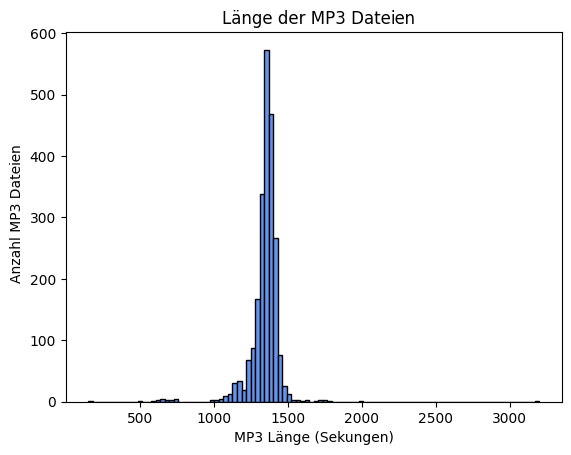
\includegraphics[width=\linewidth]{figures/mp3_length.png}

Die Transkripte der Episoden sind meißt ca. 3000 Wörter lang und benötigen ungefähr 20 KB Speicherplatz. [TODO Graphiken einfügen]







Über die API kann auch in einigen Fällen direkt ein Transkript des Audiofiles angefordert werden. 
Allerdings ist die Transkription meist nicht sehr akkurat.


Zum Beispiel steht in der Transkription des Satzes ... TODO
Das liegt daran, das die Transkriptionen mithilfe der Tools vom Fraunhofer Instituts erstellt werden, welches vermutlich veraltete Technik benutzt.



\chapter{Architektur}\label{ch:method}


\section{Mikrosystemarchitektur}

Der zweite Teil des Systems besteht darin, aus der Anfrage der Nutzenden eine passende Podcastepisode zu erstellen.
Diesen 

Dieses Projekt lässt sich zunächst in mehrere kleinen Projekte unterteilen. 
Bei einem so großen Projekt lohnt es sich eine Mikroservice Architektur anzustreben, bei der jeder Teil für sich gesehen eine Aufgabe erfüllt und nicht auf der Zuverlässigkeit eines anderen Systems beruht. 
Diese Methode wird auch divide-and-conquer genannt. 

Um das Projekt weiter einzuordnen, bietet es sich an, vorab Anforderungen an das System zu stellen. 
Da das gesamte Projekt als eine Reihe von Mikroservices umgesetzt werden soll, werden folgend für jeden Mikroservice einzelne Anforderungen gestellt: 

\section{Anforderungen}

Zunächst muss die Datengrundlage geschafft werden. 
Dafür müssen die Podcast Epsioden heruntergeladen, transkribiert und anschließend alle Sätze in der Datenbank abgespeichert werden.
Dieses System muss in der Lage dem Titel eines Podcasts bzw. der ID in der Audiothek, sämtliche noch nicht in der Datenbank gespeicherten Episoden herunterzuladen, zu transkribieren und abzuspeichern.
In der Zukunft könnte man darüber nachdenken, diesen Teil komplett auf der Serverseite der ARD Audiothek laufen zu lassen.

Das nächste Mikrosystem muss in der Lage sein, diese Transkriptdaten in eine Form umzuwandeln, in der eine Suchfunktion relevante Abschnitte aus diesen Daten extrahieren kann.
Dafür soll es die einzelnen Wörter in sinnvolle Abschnitte Gruppieren und ein Embedding für jeden Abschnitt berechnen.

Ein weiterer Service soll dann die Suchfunktion übernehmen, indem er Stichworte oder Sätze als Parameter erhält und zu diesen die eine bestimmte Anszahl an relevanten Abschnitten zurückgibt.

Diese relevanten Abschnitte können noch weiter von ChatGPT analysiert werden, um zum Besipiel eine Auswahl aus vielen Dokumenten zu treffen, die Reihenfolge der Abschnitte zu bestimmen, oder ähnliche Themen herauszufinden.

Der nächste Service muss in der Lage sein, eine Liste an Segmenten entgegenzunehmen und daraus eine Audiodatei zu erzeugen.
Dafür muss er die originaldatein an den richtigen Stellen schneiden und die Audioschnipsel zusammenfügen können.

Als letztes muss die Audiodatei ausgeliefert werden. 
Dafür soll einmal eine API implementiert werden.
Außerdem soll ein UI als Webseite aufgbaut werden, welche die Anfrage in einem Formular entgegennimmt und dann die Audiodatei ausliefert.


\section{Vorgehensweise}


Zunächst müssen die Daten gesammelt und aufbereitet werden. 
Für dieses Projekt bildet die Datengrundlage die Transkripte, bzw. Manuskripte der Podcasts der ARD-Audiothek. 
In der Audiothek selber gibt es keine Transkripte zu den Podcasts. 
Für den Podcast „radiowissen“ von bayern2 gibt es auf deren Seite die Manuskripte in PDF Format. 
Diese sind zwar inhaltlich hochqualitativ, da Sie exakte Wortwahl der Podcasts enthalten, als PDF Format sind sie allerdings schwierig maschinell auszulesen und weiterhin besitzen sie keine Zeitinformationen zu den einzelnen Wörtern. 
Die Zeitinformationen in Form von Zeitstempeln für jedes Wort sind wichtig, um die Audiofiles der Podcasts später an den richtigen Stellen zuzuschneiden. 

Ein anderer Ansatz ergibt sich, wenn man die Podcasts transkribiert. 
Die Vorteile sind, dass die Transkription auch bei Podcasts funktioniert, für die vorab kein Transkript erstellt wurde, was die Mehrzahl aller Podcasts ausmacht. 
Außerdem kann man bei einer Transkription auch gleichzeitig die Zeitstempel für jedes Wort extrahieren.

\section{Programmiersprache Python}

In dieser Arbeit wird die Programmiersprache Python verwendet.
Python zählt zu den am meißten verwendeten Programmiersprachen weltweit und ist laut dem TIOBE-Index im Jahr 2023 sogar die meißt verwendete Programmiersprache überhaupt \cite{index2023}.
In dieser Arbeit wird Python verwendet, da es Unterstützung für sehr gute Bibliotheken für Machine Learning und NLP Anwendungen gibt.
Vor allem die Unterstützung für Transformermodelle mit der Bibliothek transformers, die NLP Bibliothek SpaCy, sowie Datenverwaltungsbibliotheken wie pandas und support für SQLite Datenbanken mit sqlite sind sehr praktisch.
Dazu ist Python sehr einfach zu verstehen und rechenaufwändige Operationen wie in der transformers Bibliothek sind sehr performant in der Sprache C implementiert.





\section{Transktript Segment Ranking}

\subsection{Ählichkeitssuche lexikalisch}

\subsubsection{Keywordsuche}

Eine Möglichkeit bietet sich in der Keywordsuche. 
Hierbei wird einfach überprüft, ob sich ein Keyword in einem der Dokumente wiederfindet. Ist die möchte ein User beispielsweise einen zusammengeschnittene Podcast Episode über „Zugspitze“, so schaut das System, in welchen Episodensegmenten das Wort „Zugspitze“ auftaucht, und gibt diese zurück. 
Schwieriger wird es, wenn die Useranfrage mehrere Wörter beinhaltet. 
Möchte sich der User über das Thema „Zugspitze wandern“ informieren so müsste zunächst untersucht werden, welche Dokumente beide Worte enthalten, welche nur eines der beiden enthalten. 
Dann müsste man dementsprechend auch ein Algorithmus entwickeln, der diese dann sinnvoll hierarchisiert. 

\subsubsection{TF-IDF}

Einen solchen Ansatz bietet das TF-IDF Maß (Term Frequency – Inverse Document Frequency). 
Im Bereich des NLP verwendet man das TF-IDF Maß um zu untersuchen welche Wörter in verschiedenen Dokumenten welche Gewichtung erfahren. 
Dazu wird zunächst die TF-Matrix, also die Term Frequenzy Matrix berechnet. 
Hierbei wird erst das Vokabular ermittelt, also die Gesamtheit aller Tokens (Wörter) die es in allen Dokumenten (Transkript Segmenten) des Korpuses (alle heruntergeladenen Episoden) gibt. 
Dann wird für jedes einzelne Segment die Anzahl jeder in ihm auftretenden Tokens ermittelt. 
Für den Satz: „Auf der Zugspitze gibt es viele Wanderer, die die Zugspitze lieben“. 
In diesem Fall würde in der TF Matrix an der Stelle Zugspitze eine 2 Stehen, in der Zeile Wandern aber 0, da zwar das Wort Wanderer, aber nicht das Wort wandern vorkommt. 
Da diese beiden Worte aber sehr ähnlich sind und der User bei einer Anfrage nicht immer nach verschiedenen Versionen eines Wortes suchen will, um dann ein zufriedenstellendes Audio zu erhalten


\subsection{Sätze Normalisieren / cleanen}

Für Retrieval funktionen ist es Sinnvoll, mehrere Wörter zusammenzufassen.
Wenn man einen Algorithmus hat, der gezielt Wörter im Korpus suchen kann, ist es Wünschenswert nicht nur exakt die selben Wörter zu suchen, sondern auch verwandte Wörter.
Zum Beispiel sollte die Suche nach dem Wort "Wanderer" auch Ergebisse für die Worte "Wandererin", "Wanderung" oder "wandern" enthalten, nicht aber das Wort "Wand".

\subsubsection{Tokenisierer}

In Machine Leerning Anwendungen nutzt man dafür verschiedene Tokenisierer.
Es gibt einfache Tokenisierer, wie Whitespace Tokenisierer, die einen Text einfach an Leerzeichen teilen und die einzelnen Wörter als Tokens behandeln.
Etwas besser sind Wort Tokenizer, die auch Satzzeichen erkennen und dadurch Punkte und Kommata nicht an das Ende des vorangegangenen Wortes anhängen. 
Einen solchen Tokenizer nutzt beispielsweise spaCy, um "Linguistic Features" zu bestimmen.
Es gibt Subword tokenisierer, die Worte nocheinmal in kleinere Abschnitte teilen.
Das Byte-Pair Encoding versucht aufgrund von Statistischen Methoden, häufig vorkommende zusammenhängende Zeichenfolgen als Tokens zu identifizieren.
Diese Art Tokenizer wird zum Beispiel oft für die Eingabe bei Transformern genutzt. [Quelle]
Die Transformermodelle von OpenAI benutzen beispielsweise tiktoken als Tokenizer [Quelle], das BERT Modell von Google benutzt den WordPiece Tokenizer.



\subsubsection{Lemmatisierung vs. Stemming}

Um diese Abbildung von mehreren Worten auf ein Stammwort zu erreichen, gibt es zwei unterschiedliche Methoden:
Die Methode Stemming versucht regelbasiert Suffixe von Worten zu ersetzen, um aus Wörtern mit verschiedenen Endungen, wie zum Beispiel "Wanderer" und "Wanderung" zu einem Wort "Wander" zu reduzieren.
Der Vorteil ist, dass der Algorithmus sehr schnell agieren kann, um die Worte auf ihre Stammform zu reduzieren.
Die Nachteile sind allerdings, dass die Deutsche Sprache sehr viele verschiedene Wortkonstrukte erlaubt, die nicht alle mithilfe von einzelnen Regeln auf ein gemeinsammes Stammwort gebracht werden können. 
Zum Beispiel bei dem Plural von "Baum"; "Bäume".


\subsubsection{Kompositatrennung Pyphen vs german compound splitter}

Als weiteren Vorverarbeitungsschritt für die effiziente Keywordsuche kann man zusammengesetzte Wörter in ihre bestandteile auftrennen.
Das Vokabular des Datensazes besteht zu 61\% aus Nomen. 
Die meisten der Nomen sind zusammengesetzte Nomen, manche davon sind sehr lang, wie zum Beispiel "reichsdeputationshauptschlussakte", oder "hochgeschwindigkeitstransportmittel".
In dem ganzen Vokabular, das aus den Transkriptionen von Whisper stammt, besteht fast die Hälfte (47,8\%) aus zehn oder mehr Buchstaben.
Da für exakte Keywortsuche solche Begriffe fast nie auftreten, lohnt es sich, 



Dabei gibt es allerdings keine Möglichkeit, die verschiedenen Treffer dieser suche nach Relevanz zu hierarchisieren. Sucht man zum Beispiel nach dem Stichwort „Klimakrise“ würden dabei mehrere Stunden Material zusammenkommen [QUELLE]. 
Man könnte nun einfach die Ersten Segmente nehmen, die zusammen die vorgegebene Zeit überbrücken. Allerdings ist dieser Ansatz wenig Vielversprechend. 


\subsection{Ähnlichkeitssuche Semantisch}

\subsubsection{Embeddings}

\subsection{Ähnlichkeitsvergleiche}

Mithilfe der Embedding Vektoren können können wir Sätze finden, die zueinander Ähnlich sind. Aber was bedeutet überhaupt ähnlich? Die Vektoren des BERT Models sind 768 Dimensional, haben also 768 Gleitkommazahlen gespeichert, die zwischen -1 und 1 liegen. 
Diese Gleitkommazahlen Vektoren könnte man auch als Feature Vektoren begreifen. 
Zum Beispiel könnte die erste Zahl dieses Vektors für die Erwähnung von Professoren in dem Satz stehen (-1 für keine Professoren; 1 für viele Professoren). 
Die zweite Zahl könnte für das Thema Essen stehen (-1 für wenig mit Essen zu tun; 1 für sehr viel mit Essen zu tun). 
Damit hätte der Satz „In der Mensa gibt es jeden Tag Currywurst mit Pommes“ an der ersten Stelle vielleicht eine 0,1, weil der Begriff „Mensa“ leicht mit Uni und Professoren konnotiert wird und die zweite Stelle würde bei 0,94 liegen, da es in dem Satz offensichtlich um das Essen handelt. 
In der Realität wird das Model sehr wahrscheinlich nicht so für Menschen offensichtlichen Merkmale lernen. Ein Grund dafür ist, dass das Model vor allem pro Eintrag eine linearkombination von verschiedenen Menschenoffensichtlichen Merkmalen lernen wird, also jede Zahl eine überlagerung verschiedener Eigenschaften darstellt. 
Eine forschungsrichtung, die versucht solche Modelausgaben Menschenlesbar zu gestalten liegt in der Explainable AI

Um die Ähnlichkeit von diesem Satz zu der Frage „“ zu bestimmen nutzen wir die Cosinus distanz als Maß. Es gibt auch die Euclidische Distanz, allerdings gestaltet sich dabei das Problem der Vector Normalisierung.


Diese Komplexen semantischen Unterschiede, oder Gemeinsamkeiten zu erkennen erfordert etwas mehr Raffinesse.

Andere Distanzmaßen:
Manhatten Distanz (nur x oder y Achse)
Hamming Distanz (Anzahl verschiedener Einträge)

\subsubsection{Euclidean Similarity}

Die Euklidische Distanz von zwei Vektoren kann man über den Satz des Pythagoras berechnen.
Dafür nimmt man für jede Dimension die Differenz beider Vektoren in dieser Dimension, quadriert diese und summiert alle Quadrate zusammen, um dann die quadratwurzel darüber zu ziehen.
Für die beiden Vektoren 
$\begin{pmatrix}0\\1\end{pmatrix}$
und 
$\begin{pmatrix}-1\\0\end{pmatrix}$
wäre die

Euklidische Distanz $\frac{1}{\sqrt{2}}$, da $\sqrt{(0-(-1))^2 + (1-0)^2}=\frac{1}{\sqrt{2}}$

Dieses Distanzmaß ist sensibel gegenüber der Länge der Vektoren.
Wenn die Vektoren nicht normiert wurden, kann die Euklidische Distanz sehr groß werden und die Ergebnisse einer Ähnlichkeitssuche verfälschen.


\subsubsection{Cosinus Similarity}

Ein weiteres Ähnlichkeitsmaß kann man über den Winkel zwischen zwei Vektoren definieren.
Dieser Winkel ist unanhängig davon, wie lang die Vektoren sind, immer gleich.
Die weitverbreiteste Methode um diesen Winkel zu messen, ist über die Cosinus Ähnlichkeit.
Diese berechnet den Cosinus des Winkels und kann einfach über die Formel

$\text{cosine\_similarity}(\mathbf{a}, \mathbf{b}) = \frac{\mathbf{a} \cdot \mathbf{b}}{\|\mathbf{a}\| \|\mathbf{b}\|}$

berechnet werden.
Dabei wird für beide Vektoren zunächst das Skalarprodukt bestimmt.
Das Skalarprodukt besitzt die Eigenschaft groß zu sein, wenn beide Vektoren in ähnliche Richtungen zeigen und kleiner, wenn beide Vektoren in unterschiedliche Richtungen zeigen.
Dabei hat die Länge der unterschiedlichen Vektoren einen Einfluss auf die Größe des Skalarproduktes.
Um dieser Verzerrung entgegenzuwirken, wird das Skalarprodukt durch das Produkt der Beträge der Vektoren geteilt.
Dadurch erhält man den cosinus des Winkels zwischen diesen beiden Vektoren.

Wenn beide Vektoren vorher normiert wurden, das heißt der Betrag der Vektoren gleich Eins ist, ist die Cosinus Distanz gleich der Skalarprodukt Distanz der beiden Vektoren.
Außerdem kann in diesem Fall die Euklidische Distanz asu der Cosinus Distanz errechnet werden durch die Formel: 

$\text{Euclidean distance} = \sqrt{2 - 2 \cos(\theta)}$

\subsection{Anreichern der Segmente}

Das Ranking der einzelnen Sätze liefert eine Auswahl der besten Kandidaten für den Podcast.
Einzelne Sätze, die aus verschiedenen Podcast Episoden stammen ohne Kontext hintereinander abzuspielen bietet für den Zuhörer nur ein mäßiges Hörerlebnis. 
Es fehlt der Kontext zu den einzelnen Informationen.
Zum Besipiel bekommt man für die Suchanfrage "Geschichte Amsterdam" mit dem TF-IDF Ansatz Sätze wie "Amsterdam, das bedeutet unbeschwerte Kinderjahre" oder "Amsterdam gefiel ihm".
Die Sätze an sich bieten kaum interessante Informationen.
Dem Zuhörer stellen sich sogar noch mehr Fragen, zum Beispiel für wen Amsterdam unbeschwerte Kinderjahre bedeuten oder wem Amsterdam gefiel.

Um dem Zuhörer mehr Informationen zu geben kann man die Größe der einzelnen Segmente Anpassen.
Dazu kann man mehrere Ansätze betrachten.
Der einfachste Ansatz ist, für jeden einzelnen Satz die umgebenden Sätze davor und dahinter miteinzubeziehen.
Die Anzahl der umgebenden Sätze ist dann ein Hyperparameter dieses Systems und kann vom Nutzer durch den Parameter Segmentlänge eingestellt werden, welher die Anzahl der Sätze in einem Segment angibt.
Falls der auszuschneidende Satz am Anfang oder am Ende des Transkriptes vorkommt, und die Segmentlänge so eingestellt ist, dass mehr Sätze als möglich dem Segment hinzugefügt werden sollten, so wird das Segment an der Transkriptgrenze abgeschnitten.
Die Evaluation der besten Segmentlänge wurde in dieser Arbeit nicht ausgeführt, als defaultwert ist für die Segmentlänge 5 eingestellt.

Ein weiterer Ansatz wäre auch hier ein mächtiges LLM, wie ChatGPT zu benutzen, um die richtige Segmentlänge für jedes Segment individuell einzustellen.
Dazu kann man das LLM instruieren, aus einer sehr großen Anzahl an Kontextsätzen (zum Beispiel 50) oder dem ganzen Transkript einer Podcast Episode und der dazugehörigen Frage, die Anzahl der Kontextsätze auf das wesentliche zu beschränken.

% Dieser Ansatz würde allerdings sehr zeit- und rechenaufwändig sein.
% Wenn man als LLM ChatGPT benutzen würde, dann würden pro einzelnem Segment ca. 50 Sätze (entspricht ca. 500 Tokens) ca. 0.00025 \$ kosten entstehen.

In dieser Arbeit wurde dieser Ansatz ausprobiert mithilfe eines Promptes wie 

Je nachdem welches LLM man dafür benutzt könnten Zeit und kostenfaktoren eine Rolle spielen.


\subsection{Ranking mit ChatGPT}

Nachdem nun die Einzelnen Sätze zu gößeren Segmenten erweitert wurden, kann man auch die Reihenfolge der einzelnen Segmente anpassen.
Wenn man sich beispielsweise über die "Geschichte von Amsterdam" informieren will, kommen dazu verschiedene Ausschnitte aus der Zeit der Gründung der Niederlande, der 



\section{Audio-Zusammensetzung}


Für die Bearbeitung von Audio files in Python bietet sich das Python Modul Pydub an. Mit diesem Modul kann man ein Audiofile ähnlich wie ein Array behandeln, aus dem man nun einen Abschnitt von Sekunde 2 bis Sekunde 4 schneiden möchte. 
Für die Zeitstempel der Start und End zeit jedes Audiosegments nehmen wir die Daten aus der sortierten Ranked segments.json Datei.
Diese werden dann als extra Audiofiles abgespeichert und im nächsten Schritt wieder Zusammengesetzt.

Um die Audios nun wieder zusammenzusetzen verwenden wir das gleiche Modul Pydub. Es bieten sich mehrere Möglichkeiten an, die Audiosegmente wieder zusammenzusetzen. Man könnte die Segmente einfach ohne Pause hintereinander abspielen. Dabei folgen allerdings mehrere Probleme: 
Zum einen werden die Audiofiles nicht immer an sehr passenden Stellen getrennt, sodass manchmal mitten im Wort abgebrochen wird und das nächste Segment beginnt. 
Um dieses Problem zu lösen könnte man die Audiofiles langsam ausfaden lassen.

Außerdem sollte dem Hörer bewusst sein, dass ein Audiosegment aus einer Episode aufhört und das nächste beginnt. 
Dafür bietet sich ein kurzer Signalton zwischen den einzelnen Audiosegmenten an. 
Dieser sollte nicht nervig sein, da er dem Hörer öfter vorgespielt wird. 

Eine weitere Möglichkeit wäre, zwischen jedem Segment dem Hörer eine kurze Vorstellung der Episode und der Sprecher*in zu ermöglichen oder sogar Kontext zu dieser zu geben. 

\section{Auslieferung}

Für das Deployment dieses Tools wurde das Webframework Flask genutzt.
Flask ist ein Web Service Gateway Interface Server (WSGI), welches das bereitstellen von Webseiten über die WSGI Schnittstelle ermöglicht, welche dann von einem HTTP Server ausgeliefert werden können.
In dieser Arbeit wird dafür der WSGI HTTP Server gunicorn verwendet.
Gunicorn ist für Unix Systeme geeignet, einfach zu konfigurieren und bietet support für mehrere Worker, die mehrere Anfragen gleichzeitig bearbeiten können.

Für die Auslieferung wurde eine API und eine Webseite entwickelt.

\subsection{API}

Über die API kann der Podcast Generator einfach von anderen Anwendungen aufgerufen werden.
Die API wird aufgerufen über eine GET Request auf die unterseite /api .

Als Parameter akzeptiert die API einen String "text", welcher die Frage des Nutzers angibt.
Außerdem kann über den Parameter "time" ein Integer wert angegeben werden, welcher die Zeit des Podcasts in Minuten angibt.
Der optionale Parameter "segment-length" kann als Integer übergeben werden und bestimmt die Länge der einzelnen Segmente.

Die API gibt bei Erfolgreicher verarbeitung den Statuscode 200 zurück und liefert als Inhalt ein JSON String zurück der eine einzige Variable "url" enthält.
Diese URL verweist auf das generierte MP3 file.

\subsection{Design Webseite}

Das Design der Webseite beruht auf einem Template von https://github.com/muhammed/mini-player.
Dieses Template wurde erweitert, durch einen Suchbereich und einen Transkript Bereich.




\chapter{Evaluation verschiedener semantischer Verfahren}\label{ch:experiments}


\section{BERT Embeddings}

BERT (Bidirectional Encoder Representations from Transformers) \cite{devlin2019} ist ein auf NLP Aufgaben spezialisierter Transformer.
Er wurde von Google 2019 entwickelt und war seinerzeit das Beste Modell um verschiedene Aufgaben im Bereich des NLP zu lösen.
Unter diesen Aufgaben befinden sich Next Sentence Prediction (NSP) und Masked Language Modeling, auf das es auch trainiert wurde.
Außerdem kann man das Modell mit wenig aufwand auf andere Aufgaben finetunen und damit sehr gute Ergebnisse im Bereich der Named Entity Recognition, der Sentiment Analyse oder  

\section{Sentence Transformer Embeddings}

Das Sentence Transformer Projekt baut auf der Architektur von BERT auf. 
Es wird auch SBERT für Sentence BERT genannt. 
Unter dem 

\section{LLama2 Embeddings}

\section{Auswertung}
\chapter{Ausblick}\label{ch:outlook}

In diesem Kapitel wird ein Ausblick über verschiedene Möglichkeiten der Verbesserung des Systems erläutert.

Es bleibt abzuwarten, ob der gesamte Prozess des Information Retrievals nicht bald obsolet wird, da neuere Forschung in Mistral of Experts \cite{jiang2024}, das Retrieval über große Kontextgrößen wesentlich verbessern.
Die neuen Modelle von Gemini1.5 Pro können über 10 Millionen Token verarbeiten und haben eine außergewöhnliche Retrieval rate.

\chapter{Zusammenfassung}\label{ch:summary}

Zusammenfassend kann man sagen, dass ...




\backmatter
% \listoffigures
% \cleardoublepage

% \listoftables
% \cleardoublepage

% \renewcommand{\lstlistlistingname}{List of Listings}  % change for German thesis
% \lstlistoflistings
% \cleardoublepage

% \bibliographystyle{wmaainf}

% \bibliography{literatur}
\chapter{Anhang}\label{app:supplemental-information}

GraphQL Abfrage um alle Episoden des Podcasts "Radio Wissen" zu erhalten
Die Programset-ID verweist auf den speziellen Podcast.

\begin{verbatim}
{
    programSet(id: 5945518) {
        title
        items(
            orderBy: PUBLISH_DATE_DESC
            filter: {
            isPublished: {
                equalTo: true
            }
            }
        ) {
            
            nodes {
                title,
                audios {
                    downloadUrl
                }
            }
        }
    }
}

\end{verbatim}

\printbibliography
\printnoidxglossaries

\end{document}
